You may also watch me
\href{https://www.youtube.com/playlist?list=PLbgaMIhjbmEnaH_LTkxLI7FMa2HsnawM_}{teaching
this material} to a live audience.

\begin{quote}
For some time now I've been floating the idea of writing a book about
category theory that would be targeted at programmers. Mind you, not
computer scientists but programmers --- engineers rather than
scientists. I know this sounds crazy and I am properly scared. I can't
deny that there is a huge gap between science and engineering because I
have worked on both sides of the divide. But I've always felt a very
strong compulsion to explain things. I have tremendous admiration for
Richard Feynman who was the master of simple explanations. I know I'm no
Feynman, but I will try my best. I'm starting by publishing this preface
--- which is supposed to motivate the reader to learn category theory
--- in hopes of starting a discussion and soliciting feedback.
\end{quote}

I will attempt, in the space of a few paragraphs, to convince you that
this book is written for you, and whatever objections you might have to
learning one of the most abstract branches of mathematics in your
``copious spare~time'' are totally unfounded.

My optimism is based on several observations. First, category theory is
a treasure trove~of extremely useful programming ideas. Haskell
programmers have been tapping this resource~for a long time, and the
ideas are slowly percolating into other languages, but this process is
too slow. We need to speed it up.

Second, there are many different kinds of math, and they appeal to
different audiences. You might be allergic to calculus or algebra, but
it doesn't mean you won't enjoy category theory. I would go as far as
to~argue~that category theory is the kind of math that is particularly
well suited for the minds of programmers. That's because category theory
--- rather than dealing with particulars --- deals with structure. It
deals with the kind of structure that makes programs composable.

Composition is at the very root of category theory --- it's part of the
definition of the category itself. And I will argue strongly that
composition is the essence of programming. We've been composing things
forever, long before some great engineer came up with the idea of a
subroutine. Some time ago the principles of structural programming
revolutionized programming~because they made blocks of code composable.
Then came object oriented programming, which is all about composing
objects. Functional programming is not only about composing functions
and algebraic data structures --- it makes concurrency composable ---
something that's virtually impossible with other programming paradigms.

Third, I have a secret weapon, a butcher's knife, with which I will
butcher math to make it more palatable to programmers. When you're a
professional mathematician, you have to be very careful to get all your
assumptions straight, qualify every statement properly, and construct
all your proofs rigorously. This makes mathematical papers and books
extremely hard to read for an outsider. I'm a physicist by training, and
in physics we made amazing advances using informal reasoning.
Mathematicians laughed at the Dirac delta function, which was made up on
the spot by the great physicist P. A. M. Dirac to solve some
differential equations. They stopped laughing when they discovered a
completely new branch of calculus called distribution theory that
formalized Dirac's insights.

Of course when using hand-waving arguments you run the risk of saying
something blatantly wrong, so I will try to make sure that there is
solid mathematical theory behind informal arguments in this book. I do
have a worn-out copy of Saunders Mac Lane's \emph{Category Theory for
the Working Mathematician} on my nightstand.

Since this is category theory \emph{for programmers} I will illustrate
all major concepts using computer code. You are probably aware that
functional languages are closer to math than the more popular imperative
languages. They also offer more abstracting power. So a natural
temptation would be to say: You must learn Haskell before the bounty of
category theory becomes available to you. But that would imply that
category theory has no application outside of functional programming and
that's simply not true. So I will provide a lot of C++ examples.
Granted, you'll have to overcome some ugly syntax, the patterns might
not stand out from the background of verbosity, and you might be forced
to do some copy and paste in lieu of higher abstraction, but that's just
the lot of a C++ programmer.

But you're not off the hook as far as Haskell is concerned. You don't
have to become a Haskell programmer, but you need it as a language for
sketching and documenting ideas to be implemented in C++. That's exactly
how I got started with Haskell. I found its terse syntax and powerful
type system a great help in understanding and implementing C++
templates, data structures, and algorithms. But since I can't expect the
readers to already know Haskell, I will introduce it slowly and explain
everything as I go.

If you're an experienced programmer, you might be asking yourself: I've
been coding for so long without worrying about category theory or
functional methods, so what's changed? Surely you can't help but notice
that there's been a steady stream of new functional features invading
imperative languages. Even Java, the bastion of object-oriented
programming, let the lambdas in C++ has recently been evolving at a
frantic pace --- a new standard every few years --- trying to catch up
with the changing world. All this activity is in preparation for a
disruptive change or, as we physicist call it, a phase transition. If
you keep heating water, it will eventually start boiling. We are now in
the position of a frog that must decide if it should continue swimming
in increasingly hot water, or start looking for some alternatives.

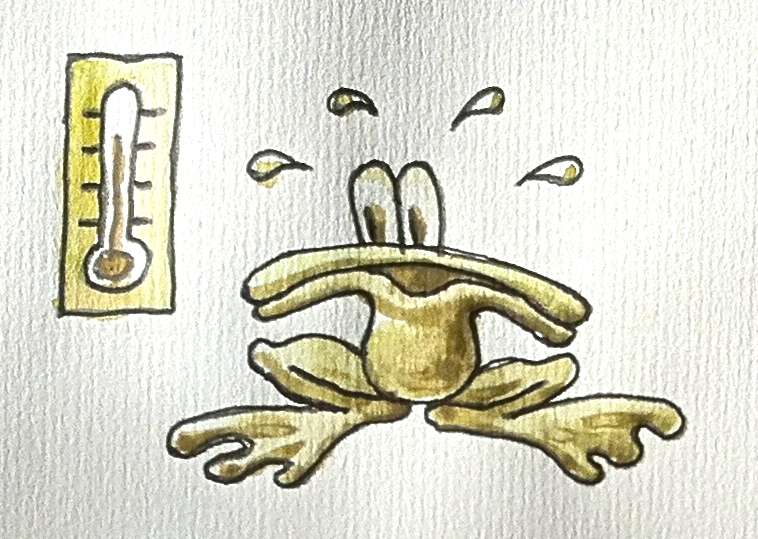
\includegraphics[width=3.12500in]{images/img_1299.jpg}

One of the forces that are driving the big change is the multicore
revolution. The prevailing programming paradigm, object oriented
programming, doesn't buy you anything in the realm of concurrency and
parallelism, and instead encourages dangerous and buggy design. Data
hiding, the basic premise of object orientation, when combined with
sharing and mutation, becomes a recipe for data races. The idea of
combining a mutex with the data it protects is nice but, unfortunately,
locks don't compose, and lock hiding makes deadlocks more likely and
harder to debug.

But even in the absence of concurrency, the growing complexity of
software systems is testing the limits of scalability of the imperative
paradigm. To put it simply, side effects are getting out of hand.
Granted, functions that have side effects are often convenient and easy
to write. Their effects can in principle be encoded in their names and
in the comments. A function called SetPassword or WriteFile is obviously
mutating some state and generating side effects, and we are used to
dealing with that. It's only when we start composing functions that have
side effects on top of other functions that have side effects, and so
on, that things start getting hairy. It's not that side effects are
inherently bad --- it's the fact that they are hidden from view that
makes them impossible to manage at larger scales. Side effects don't
scale, and imperative programming is all about side effects.

Changes in hardware and the growing complexity of software are forcing
us to rethink the foundations of programming. Just like the builders of
Europe's great gothic cathedrals we've been honing our craft to the
limits of material and structure. There is an unfinished gothic
\href{http://en.wikipedia.org/wiki/Beauvais_Cathedral}{cathedral in
Beauvais}, France, that stands witness to this deeply human struggle
with limitations. It was intended to beat all previous records of height
and lightness, but it suffered a series of collapses. Ad hoc measures
like iron rods and wooden supports keep it from disintegrating, but
obviously a lot of things went wrong. From a modern perspective, it's a
miracle that so many gothic structures had been successfully completed
without the help of modern material science, computer modelling, finite
element analysis, and general math and physics. I hope future
generations will be as admiring of the programming skills we've been
displaying in building complex operating systems, web servers, and the
internet infrastructure. And, frankly, they should, because we've done
all this based on very flimsy theoretical foundations. We have to fix
those foundations if we want to move forward.

\hypertarget{attachment_3472}{}
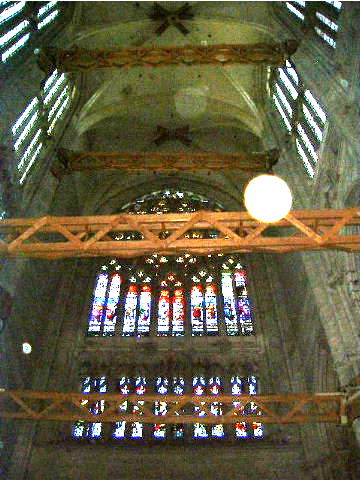
\includegraphics[width=2.34375in]{images/beauvais_interior_supports.jpg}

Ad hoc measures preventing the Beauvais cathedral from collapsing

Next:
\href{https://bartoszmilewski.com/2014/11/04/category-the-essence-of-composition/}{Category:
The Essence of Composition}.

\href{https://twitter.com/BartoszMilewski}{Follow @BartoszMilewski}
